\documentclass[border=10pt]{standalone}
\usepackage{tikz}
\usetikzlibrary{calc, positioning, arrows.meta}

\begin{document}
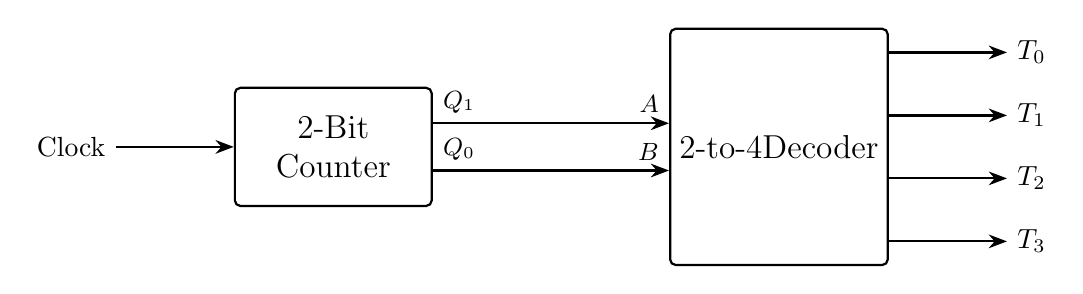
\begin{tikzpicture}[
    >=Stealth, 
    thick, 
    box/.style={draw, minimum width=2.5cm, minimum height=1.5cm, font=\large, rounded corners=2pt},
    label_font/.style={font=\small}
]

    % Components
    % 2-bit Counter
    \node[box, align=center] (counter) at (0,0) {2-Bit\\Counter};
    
    % 2-to-4 Decoder
    \node[box, minimum width=2.0cm, minimum height=3.0cm, right=3cm of counter] (decoder) {2-to-4\\Decoder};
    
    % Connections
    
    % Clock to Counter
    \draw[->] ($(counter.west) + (-1.5, 0)$) node[left] {Clock} -- (counter.west);
    
    % Counter to Decoder
    % Q0 -> B (LSB?)
    % Q1 -> A (MSB?)
    % Usually input labels on Decoder: A, B or I0, I1. 
    % Let's use A (MSB), B (LSB) or just lines.
    
    \draw[->] ($(counter.east) + (0, 0.3)$) node[above right, label_font] {$Q_1$} -- ($(decoder.west) + (0, 0.3)$) node[above left, label_font] {$A$};
    \draw[->] ($(counter.east) + (0, -0.3)$) node[above right, label_font] {$Q_0$} -- ($(decoder.west) + (0, -0.3)$) node[above left, label_font] {$B$};
    
    % Decoder Outputs (Timing Signals)
    % 4 outputs: T0, T1, T2, T3
    
    \foreach \i in {0,1,2,3} {
        \pgfmathsetmacro{\ypos}{1.2 - \i*0.8}
        \coordinate (out_\i) at ($(decoder.east) + (0, \ypos)$);
        \draw[->] (out_\i) -- ++(1.5, 0) node[right] {$T_\i$};
    }
    
    % Optional: Add bubbling or active low notation if needed, but usually Timing signals are Active High pulses in this context. Use straight lines.

\end{tikzpicture}
\end{document}
